% Created 2023-03-24 sex 17:25
% Intended LaTeX compiler: pdflatex
\documentclass[11pt]{article}
\usepackage[utf8]{inputenc}
\usepackage[T1]{fontenc}
\usepackage{graphicx}
\usepackage{longtable}
\usepackage{wrapfig}
\usepackage{rotating}
\usepackage[normalem]{ulem}
\usepackage{amsmath}
\usepackage{amssymb}
\usepackage{capt-of}
\usepackage{hyperref}
\usepackage{blindtext}
\usepackage{subcaption}
\usepackage{titling}
\usepackage{titlesec}
\usepackage{amsmath, amsfonts, amssymb}
\usepackage{multicol}
\usepackage{gensymb}
\usepackage{cancel}
\usepackage{siunitx}
\usepackage{colortbl,hhline}
\usepackage[brazil, american]{babel}
\usepackage[numbers]{natbib}
\usepackage{indentfirst}
\usepackage{graphicx}
\usepackage{siunitx}
\usepackage{chemfig}
\usepackage[backend=bibtex,bibencoding=ascii,style=chem-angew,citestyle=numeric-comp,sorting=none]{biblatex}
\usepackage{tikz}
\usetikzlibrary{arrows}
\usepackage[controls]{animate}
\usepackage{color}
\usepackage{epigraph}
\usepackage{empheq}
\usepackage{indentfirst}
\usepackage[theorems,skins]{tcolorbox}
\usepackage[svgnames]{xcolor}
\usepackage[explicit]{titlesec}
\usepackage[backend=bibtex]{biblatex}

\usepackage{physics}
\usepackage[svgnames]{xcolor}
\usepackage{framed}
\DeclareMathOperator{\sen}{sen}
\usepackage[margin=0.8in]{geometry}
\titleformat{\section}{\Large\bfseries}{\thesection}{2.5em}{}
\titlespacing{\section}{0em}{1.5em}{1.5em}
\titleformat{\subsection}{\large\bfseries}{\thesection}{2.5em}{}[\hrule]
\titlespacing{\section}{0em}{1.5em}{1.5em}
\author{Edgard Macena Cabral}
\date{Março 2023}
\title{\href{https://edisciplinas.usp.br/pluginfile.php/7581904/mod\_resource/content/1/projeto-fiscompII-primeiro-2023-completo.pdf}{ANÁLISE ESPECTRAL POR\\  \\ TRANSFORMADAS DE FOURIER}\\\medskip
\large Edgard Macena Cabral Nº 11820833 \\  Março 2023}
\hypersetup{
 pdfauthor={Edgard Macena Cabral},
 pdftitle={\href{https://edisciplinas.usp.br/pluginfile.php/7581904/mod\_resource/content/1/projeto-fiscompII-primeiro-2023-completo.pdf}{ANÁLISE ESPECTRAL POR\\  \\ TRANSFORMADAS DE FOURIER}},
 pdfkeywords={},
 pdfsubject={A GNU Emacs notebook demonstration},
 pdfcreator={Emacs 28.2 (Org mode 9.6.1)}, 
 pdflang={English}}
\begin{document}

\maketitle
\begin{abstract}
Nessa tarefa, buscamos analisar a Transformada Discreta de Fourier sem nenhuma aceleração. Criamos um programa que realiza a transformada e outro que realiza sua inversa.
Observamos que, para alguns casos, essas operações são bem comportadas, e conseguimos recuperar o sinal sem dificuldades.
Observamos também que, para outras sinais obtivemos um reflexo em torno da frequência de Nyquist, provando que a maior frequência que podemos obter com a transformada é \(\frac{1}{2\Delta t}\).
Por fim, vimos a relação entre o número N de pontos e o tempo de 50 execuções do programa.
\end{abstract}
\section*{Introdução}
\label{sec:orgbcf407c}
A transformada de Fourier é uma transformação que nos leva do espaço das amplitude de um sinal para um espaço de frequências. Para sinais contínuos, podemos escrever:

\begin{latex}
\begin{equation}
Y(f) = \int^{\infty}_{-\infty}y(t)e^{2\pi f i t}
\end{equation}
\end{latex}

Porém, na física experimental, da análise da luminosidade de estrelas na busca de exoplanetas ao estudo do movimento de um pêndulo no laboratório de física I, trabalhamos essencialmente com dados discretos.

Para adequar a transformada aos dados laboratoriais, usamos as substituições \(t_j = j\Delta t\), \(f_k = \frac{k}{N\Delta t}\), que nos dão:

\begin{latex}
\begin{equation}
\label{eq:Transformada discreta}
Y_k = \sum_{j=0}^{j < N/2} y_j e^{2\pi jk i/N}
\end{equation}
\end{latex}

Conseguimos também obter a inversa através de

\begin{latex}
\begin{equation}
\label{eq:Transformada inversa discreta}
y_j = \frac{1}{k}\sum_{k=0}^{k < N/2} Y_ke^{-2\pi jk i/N}
\end{equation}
\end{latex}

Nessas equações, a razão de irmos apenas até \(k < N/2\) está ligada a frequência de Nyquist, que pode ser entendida como a frequência associada ao menor comprimento de onda que pode formar um modo fundamental entre pontos de data consecutivos.

Caso a frequência do sinal seja maior que a frequência de Nyquist, o gráfico, obtemos um pico relacionada à reflexão da verdadeira frequência do sinal com a de Nyquist.

\begin{latex}
\begin{equation}
\label{eq:Frequência encontrada}
  f_{encontrada} = 2f_{Nyquist} - f_{verdadeira}
\end{equation}
\end{latex}

Como já dito, transformadas de Fourier são amplamente usadas na Física, então é importante que possamos tê-la eficientemente.
Podemos estimar com facilidade a ordem do tempo de execução. Temos \(N\) termos, cada um dos quais é calculado com uma soma de \(\frac{N}{2}\) termos. A ordem do tempo de execução é então da ordem de \textasciitilde{}\(N^2\).

\section*{Geração de dados}
\label{sec:orgdd53280}
Para gerar os dados, usamos a equação a seguir:
\begin{latex}
\begin{equation}
y_{i} = a_{1}\cos{(\omega_{1}t_{i})} + a_{2}\sen(\omega_{2}t_{i})
\end{equation}
$$t_{i} = i\Delta t,\ \ i = 1, \cdots, N$$
\end{latex}

Que foi executada no programa:

\begin{verbatim}
program gerarSinais
    implicit none
    real*8, parameter :: pi = 3.1415926537989
    real*8 :: a1, a2, w1, w2, dt
    integer :: N
    ! (a) N = 200, ∆t = 0.04, a1 = 2, a2 = 4, ω1 = 4πHz, ω2 = 2.5πHz
    ! (b) N = 200, ∆t = 0.04, a1 = 3, a2 = 2, ω1 = 4πHz, ω2 = 2.5πHz
    ! (c) N = 200, ∆t = 0.4, a1 = 2, a2 = 4, ω1 = 4πHz, ω2 = 0.2πHz
    ! (d) N = 200, ∆t = 0.4, a1 = 3, a2 = 2 ω1 = 4πHz, ω2 = 0.2πHz

    call escreveSinal(200, 0.04d0, 2.d0, 4.d0, 4.d0*pi, 2.5d0, "a")
    call escreveSinal(200, 0.04d0, 3.d0, 2.d0, 4.d0*pi, 2.5d0, "b")
    call escreveSinal(200, 0.4d0, 2.d0, 4.d0, 4.d0*pi, 0.2d0, "c")
    call escreveSinal(200, 0.4d0, 3.d0, 2.d0, 4.d0*pi, 0.2d0, "d")
end program gerarSinais


subroutine escreveSinal(N, dt, a1,  a2, w1, w2, label)
    real*8, intent(in) :: a1, a2, w1, w2, dt
    integer, intent(in) :: N
    char*8, intent(in) :: label
    real*8 :: calculaSinal
    integer :: i

    open(1, file="saida-2-"//label)

    do i = 1, N
        write(1, *) i*dt, calculaSinal(i*dt, a1, a2, w1, w2)
    end do

    close(1)

end subroutine escreveSinal


function calculaSinal(t, a1, a2, w1, w2) result(retval)
    real*8, intent(in) :: a1, a2, w1, w2, t
    real*8 :: retval
    retval = a1*cos(w1*t) + a2*sin(w2*t)

end function calculaSinal
\end{verbatim}

O programa foi executado sobre as séries de parâmetros

$$(a)\ \ N = 200, \Delta t = 0,04,\ a_1 = 2,\ a_2 = 4,\ \omega_1 = 4\pi Hz,\ \omega_2 = 2,5\pi Hz$$
$$(b)\ \ N = 200, \Delta t = 0,04,\ a_1 = 3,\ a_2 = 2, \omega_1 = 4\pi Hz,\ \omega_2 = 2,5\pi Hz$$
$$(c)\ \ N = 200, \Delta t = 0,4,\ a_1 = 2,\ a_2 = 4,\ \omega_1 = 4\pi Hz,\ \omega_2 = 0,2\pi Hz$$
$$(d)\ \ N = 200, \Delta t = 0,4,\ a1 = 2,\ a2 = 4, ω1 = 4\pi Hz,\ ω2 = 2,5\pi Hz$$

Os resultados estão no gráfico a seguir

\begin{figure}[htbp]
\centering
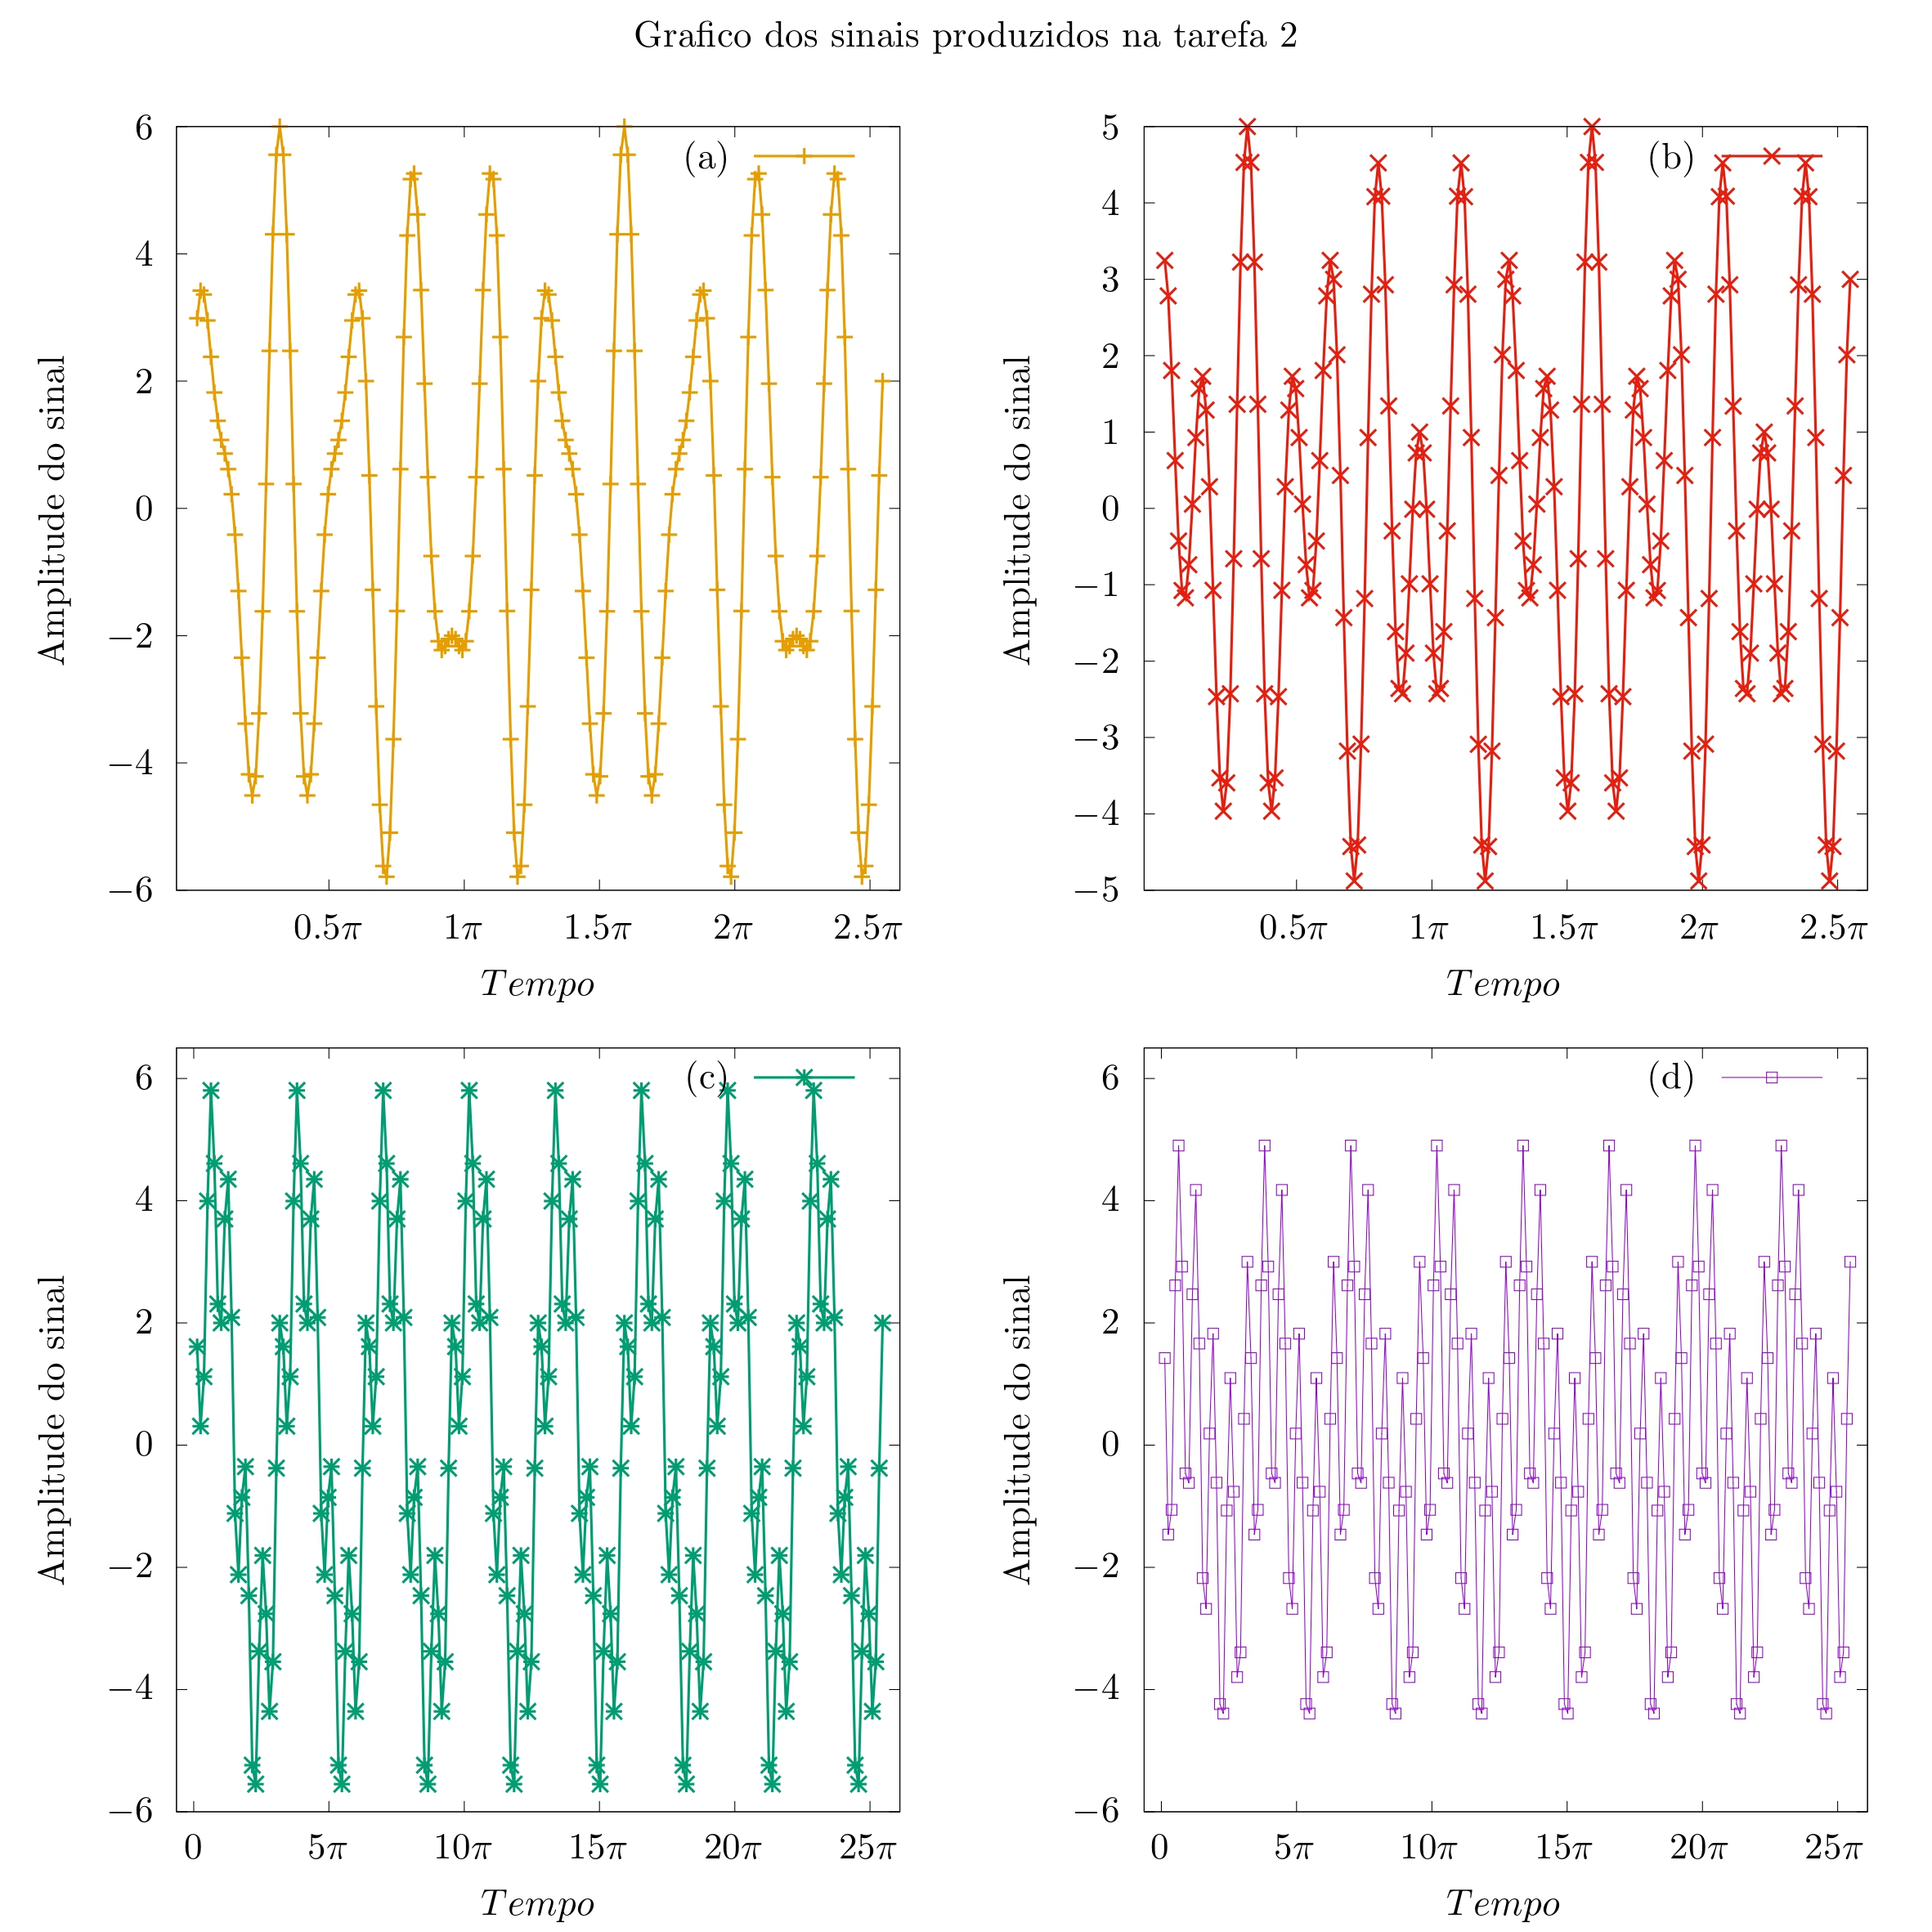
\includegraphics[width=13cm,height=13cm]{graficos/tarefa-2-graf-11820833.jpg}
\caption{Sinais gerados para os testes seguintes.}
\end{figure}

Notamos que as séries representam uma boa variedade de sinais.
A séries \((a)\) e \((b)\) são parecidas em termos de frequências, mas as amplitudes diferentes implicam em formatos bastantes diferentes, mesmo compartilhando alguns picos e vales, com algo parecido entre as séries \((c)\) e \((d)\).
Ao mesmo tempo \((a)\) e \((c)\) têm mesma amplitude, o que não chega a fazer uma série parecida, pelos picos e vales serem bastante distintos, com o mesmo ocorrendo entre a \((b)\) e \({d}\)


\section*{Transformada de Fourier}
\label{sec:orgae7ed45}

Para a Transformada de Fourier, usamos o programa a seguir:
\begin{verbatim}
program gerarEspacoFrequencias
    implicit none
    real*8, dimension(200) :: y_t
    real*8 :: dt
    integer :: N
    call leTabela(dt, y_t, N)
    call escreveFrequencias(y_t, dt, N)


end program gerarEspacoFrequencias

subroutine leTabela(dt, y_t, N)
    real*8, dimension(200), intent(out) :: y_t
    real*8, intent(out) :: dt
    integer, intent(out) :: N
    real*8 :: ignorada
    integer :: i

    open(1, file="data.in")

    do i = 1, 200
        read(1,*, end=10) ignorada, y_t(i)
        if ( i == 1 ) then
            dt = ignorada
        end if
10  end do
    close(1)

    N = i - 1

end subroutine leTabela

subroutine escreveFrequencias(y_t, dt, label, N)
    real*8, dimension(200), intent(in) :: y_t
    real*8, intent(in) :: dt
    integer :: k, N, M
    complex*16 :: Yk, currYk
    M = floor((N-1)/2.d0)

    open(2, file="data.out")
    do k = 1, M
        currYk = Yk(k, y_t, N)
        write(2,*) k/(200*dt), real(currYk), aimag(currYk)
    end do
    close(2)
end subroutine escreveFrequencias

function Yk(k, y_t, N)
    integer, intent(in) :: k
    integer, intent(in) :: N
    real*8, dimension(200):: y_t
    complex*16 :: Yk, i = (0,1)
    real*8, parameter :: pi = 3.1415926537989
    integer :: j
    Yk = (0,0)
    somatoria : do  j = 1, N
        Yk = Yk + y_t(j)*exp(2.d0*pi*i*j*k/N)
    end do somatoria

end function Yk
\end{verbatim}

Desse programa, produzimos, para os nossos sinais, os seguintes gráficos de espectro:

\begin{center}
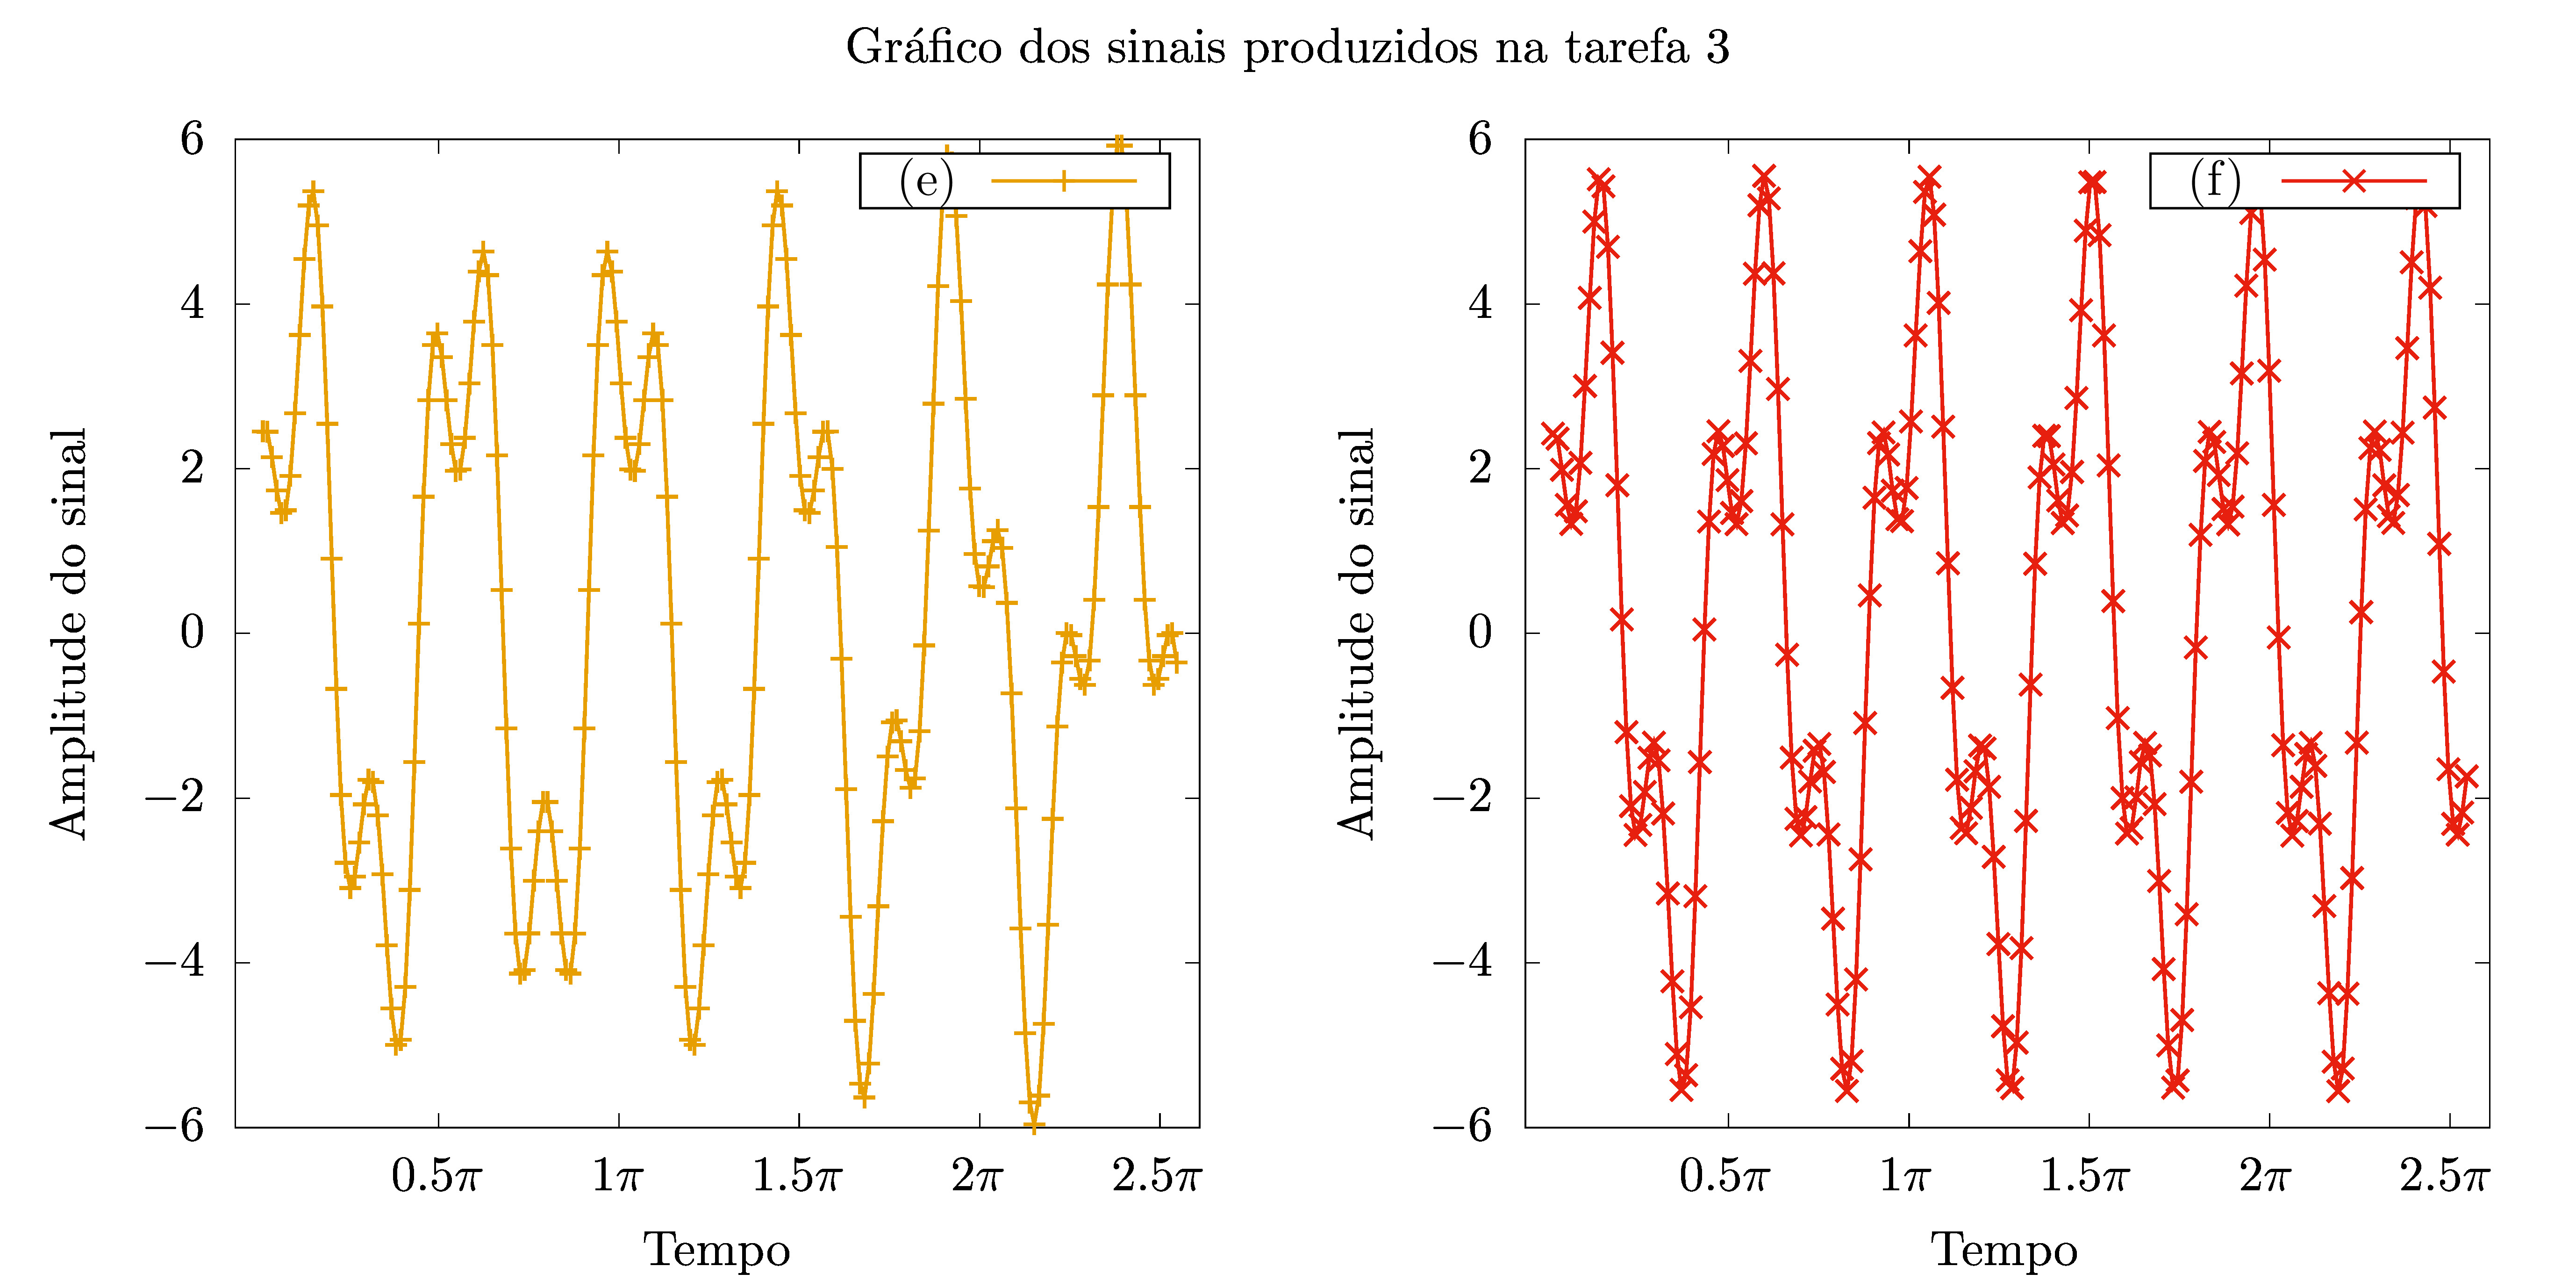
\includegraphics[width=.9\linewidth]{graficos/tarefa-3-graf-1-11820833.jpg}
\end{center}

O gráfico mostrado aqui foi produzido de maneira a reforçar os pontos onde temos os dados são relevantes. Nele, podemos ver o que as frequências dos sinais \((a)\) e \((b)\) foram recuperados sem dificuldades. Já para série \((c)\) e \((d)\), vemos que não conseguimos recuperar a frequência angular de \(4\pi Hz\) (\(2Hz\) em frequência linear).

Isso ocorre pois essa frequência está bem acima da máxima que Nyquist. De fato, fazendo
$$f_{Nyquist} = \frac{1}{2\cdot 0,4}$$

$$f_{Nyquist} = 1,25Hz$$

Podemos refletir nossa frequência \(2Hz\) em torno de Nyquist através de \((4)\) para obter

$$f_{encontrada} = 0,5Hz = \pi\Hz \textbf(frequência angular)$$

\section*{Transformada Inversa}
\label{sec:org3ce38e4}

Usamos, seguindo a \((3)\), o programa

\begin{verbatim}
program gerarEspacoAmplitude
    implicit none
    complex*16, dimension(100) :: Yk
    integer :: N

    read(*,*) label
    call leTabela(N, Yk)
    call escreveAmplitude(Yk, N, label)

end program gerarEspacoAmplitude


subroutine leTabela(N, Yk)
    real*8 ::  ignorada, Yk_real, Yk_imaginaria
    complex*16, dimension(100), intent(out) :: Yk
    integer, intent(out) :: N
    integer :: i

    open(1, file="../tarefa-1/data.out")

    do 10 i = 1, 100
        read(1,*) ignorada, Yk_real, Yk_imaginaria
        Yk(i) = complex(Yk_real, Yk_imaginaria)
 10 end do
        N = i
end subroutine leTabela

subroutine escreveAmplitude(Yk, N)
    complex*16, dimension(100), intent(in) :: Yk
    real*8 :: dt = 0.04d0
    integer :: j
    complex*16 :: y_j, curr_y_j

    open(1, file="saida-4-11820833")
    do j = 1, 2*(N + 1)
        curr_y_j = y_j(j, N, Yk)
        write(1,*) j*dt, real(curr_y_j)
    end do
    close(1)

end subroutine escreveAmplitude

function y_j(j, N, Yk)
    integer, intent(in) :: j
    complex*16, dimension(100), intent(in):: Yk
    integer, intent(in) :: N
    complex*16:: i = (0,1)
    complex*16 :: y_j
    real*8, parameter :: pi = 3.1415926537989
    integer :: k

    somatoria : do  k = 1, 100
        y_j = y_j + Yk(k)*exp(-2.d0*pi*i*j*k/(2*(N+1)))
    end do somatoria

    y_j = y_j/N

end function y_j
\end{verbatim}

Obtivemos, para a série \((a)\), o gráfico a seguir

GRAFICO

Nele, observamos uma boa sobreposição entre a nossa série original e a recuperada pela nossa inversa, demonstrando a precisão do Método de Fourier

\section*{Tempo de Execução}
\label{sec:org675428c}

Como comentando na introdução, é esperado que o tempo de execução seja da ordem de \(N^2\). 
Para comprovarmos isso, fizemos um programa que executa a Transformada de Fourier sobre o sinal
\begin{latex}
\begin{equation}
\label{eq: sinais usado pros testes}
\Delta t = 0,04,\ a_1 = 2,\ a_2 = 4,\ \omega_1 = 4\pi Hz,\ \omega_2 = 2,5\pi Hz
\end{equation}
\end{latex}
Para \(N = 50,\ 100,\ 200,\ 400\).

Para monitorarmos o tempo de execução de cada N, usamos o módulo de cpu\textsubscript{time} sobre 50 execuções da transformada para cada N, e depois tiramos a média aritmética.
O código foi basicamente o do programa de Transformada, com as alterações girando em torno da contagem de tempo e das saídas

\begin{verbatim}

program tempoPorN
   implicit none
   real*8 :: t_inicio, t_fim, delta_t
   integer :: i, j, N = 50
   character*24, dimension(4) :: files
   files(1) = "tarefa-5-050-11820833.in"
   files(2) = "tarefa-5-100-11820833.in"
   files(3) = "tarefa-5-200-11820833.in"
   files(4) = "tarefa-5-400-11820833.in"

   open(2, file="../dados/tarefa-5-11820833.out")
   do i = 1, 4
      call cpu_time(t_inicio)
      do j = 1, 20
         call gerarEspacoFrequencias(files(i))
      end do
      call cpu_time(t_fim)
      delta_t = (t_fim - t_inicio)/10.d0
      write(2, *) N, delta_t, sqrt(delta_t) 
      N = N*2
   end do
end program tempoPorN

subroutine gerarEspacoFrequencias(fileName)
   implicit none
   real*8, dimension(400) :: y_t
   real*8 :: dt
   character*24 :: fileName
   integer :: N
   call leTabela(fileName, dt, y_t, N)
   call calculaFrequencias(y_t, dt, N)

end subroutine gerarEspacoFrequencias

subroutine leTabela(fileName, dt, y_t, N)
   character*24, intent(in) :: fileName
   real*8, dimension(400), intent(out) :: y_t
   real*8, intent(out) :: dt
   integer, intent(out) :: N
   real*8 :: ignorada
   integer :: i

   open(1, file="../dados/"//fileName)

   do i = 1, 400
      read(1,*, end=1) ignorada, y_t(i)
      if ( i == 1 ) then
         dt = ignorada
      end if
   end do
  
1  close(1)

   N = i - 1
end subroutine leTabela

subroutine calculaFrequencias(y_t, dt, N)
   real*8, dimension(400), intent(in) :: y_t
   real*8, intent(in) :: dt
   integer :: k, N, M
   complex*16 :: Yk, currYk
   M = floor((N-1)/2.d0)

   do k = 1, M
      currYk = Yk(k, y_t, N)
      write(1,*) k/(200*dt), real(currYk), aimag(currYk)
   end do
end subroutine calculaFrequencias

function Yk(k, y_t, N)
   integer, intent(in) :: k
   integer, intent(in) :: N
   real*8, dimension(400):: y_t
   complex*16 :: Yk, i = (0,1)
   real*8, parameter :: pi = 3.1415926537989
   integer :: j
   Yk = (0,0)
   somatoria : do  j = 1, N
      Yk = Yk + y_t(j)*exp(2.d0*pi*i*j*k/N)
   end do somatoria

end function Yk

\end{verbatim}
\end{document}